\chapter{Epidemiological Modelling}

Researchers have developed compartmental epidemiological models to study the
behaviour and characteristics of disease spread and eradication. Compartmental
models simplify the dynamics of a disease down to a mathematically
representable form. By determining the parameters within a model,
it is possible to facilitate an understanding of
how the modelled disease spreads and assess the effectiveness of
differing disease interventions (such as treatments or vaccinations)
without large long-term trials. Models can also simulate various
scenarios, such as increases or decreases in viral transmission.

Simple compartmental disease models assume individuals can only be in one of
a finite number of states (which are called compartments). These compartments
usually correspond to a state of disease. A standard compartmental model may
include: \begin{itemize}
    \item $S$ - Susceptible: at risk of contracting the disease
    \item $E$ - Exposed: contracted the disease but not infecting other
          individuals
    \item $I$ - Infectious (also called Infected): at risk of infecting others
          with the disease
    \item $R$ - Recovered: no longer infectious and incapable of being reinfected.
\end{itemize}

\begin{figure}[htbp]
    \centering
    \begin{subfigure}[b]{0.18\textwidth}
        \begin{tikzpicture}[thick]
            \node[draw, minimum size=0.8cm] (S) {$S$};
            \node[draw, right=of S, minimum size=0.8cm] (I) {$I$};
            \draw[->] (S) edge[in = 160, out = 20] node
            [midway, label=above:{$\lambda_t$}] (lambda) {} (I);
            \draw[->] (I) edge[in = 340, out = 200] node
            [midway, label=below:{$\gamma$}] (gamma) {} (S);
            \draw[->, dashed, ruby] (I) edge[in = 45, out = 90] (lambda);
            % \draw (current bounding box.south east) rectangle
            % (current bounding box.north west);
        \end{tikzpicture}
        \caption{$SIS$ model}\label{fig:SIS_model}
    \end{subfigure}%
    \hfill%
    \begin{subfigure}[b]{0.19\textwidth}
        \begin{tikzpicture}[thick]
            \node[draw, minimum size=0.8cm] (S) {$S$};
            \node[draw, right=of S, minimum size=0.8cm] (I) {$I$};
            \draw[->] (S) edge node [midway, label=above:{$\lambda_t$}]
            (lambda) {} (I);
            \draw[->, dashed, ruby] (I) edge[in = 270, out = 225] (lambda);
            \node[above=of S] (mu) {};
            \node[below=of S] (S_nu) {};
            \node[below=of I] (I_nu) {};
            \draw[->] (mu) edge node [midway, label=left:{$\mu$}] () {} (S);
            \draw[->] (S) edge node [midway, label=left:{$\nu$}] () {} (S_nu);
            \draw[->] (I) edge node [midway, label=left:{$\nu + \gamma$}] () {}
            (I_nu);
            % \draw (current bounding box.south east) rectangle
            % (current bounding box.north west);
        \end{tikzpicture}
        \caption{$SI$ with demography model}\label{fig:SI_demog_model}
    \end{subfigure}%
    \hfill%
    \begin{subfigure}[b]{0.42\textwidth}
        \begin{tikzpicture}[thick]
            \node[draw, minimum size=0.8cm] (S) {$S$};
            \node[draw, minimum size=0.8cm, right=of S] (E) {$E$};
            \node[draw, minimum size=0.8cm, right=of E] (I) {$I$};
            \node[draw, minimum size=0.8cm, right=of I] (R) {$R$};
            \draw[->] (S) edge node [midway, label=above:{$\lambda_t$}]
            (lambda) {} (E);
            \draw[->] (E) edge node [midway, label=above:{$\sigma$}]
            (sigma) {} (I);
            \draw[->] (I) edge node [midway, label=above:{$\gamma$}]
            (r) {} (R);
            \draw[->, dashed, ruby] (I) edge[in = 270, out = 270] (lambda);
            % \draw (current bounding box.south east) rectangle
            % (current bounding box.north west);
        \end{tikzpicture}
        \caption{$SEIR$ model}\label{fig:SEIR_model}
    \end{subfigure}%
    \caption[{
        $SIS,$ $SI$ with demography, and $SEIR$ model schematics
    }]{
        Some simple model schematics with varying numbers of compartments: $S$
        (susceptible), $E$ (exposed), $I$ (infectious) and $R$ (recovered). The
        force of infection $\lambda_t$ is usually a function of $I_t$, depicted
        by the dashed red lines. $\mu$ and $\nu$ are natural birth and death
        rates, respectively. $\gamma$ is the rate of progression out of the
        infectious state. In each of these models, the physical interpretation
        differs slightly. In the $SIS$ and $SEIR$ models, it is the rate at
        which individuals move from infectious to susceptible again or into
        lifelong immunity, whereas, in the $SI$ with demography model, it can be
        interpreted as the increase in the death rate attributable to
        disease-induced mortality. $\sigma$ is the rate of progression from a
        state of latent infection to becoming infectious.
    }\label{fig:simple_models}
\end{figure}

The number of people in each compartment at time $t$ is a (possibly
non-deterministic) function of time $t,$ which we indicate as a subscript $t$
(e.g., $S_t$ is the number of susceptibles at time $t$). Models are typically
described by the compartments they contain. The $SIS$ model
depicted in Figure \ref{fig:SIS_model} consists of a susceptible compartment
$S$ and an infectious compartment $I$. In this model, individuals
who recover from infection are immediately susceptible to reinfection,
as is the case
with most sexually transmitted diseases \parencite[56]{keeling_modeling_2008}.
Movement between the two compartments is determined
by the force of infection $\lambda_t$ and rate of recovery $\gamma.$

The $SI$ with demography model depicted in Figure \ref{fig:SI_demog_model} is
used to model diseases
that infect the individual until death, such as bovine spongiform
encephalopathy (BSE), commonly known as mad cow disease
\parencite{hagenaars_epidemiological_2006}.
In addition to the rates in the $SIS$ model, $\mu$ and $\nu$ are birth and
death rates, respectively. $\gamma$ becomes the rate of disease-induced 
mortality.

The $SEIR$ model in Figure \ref{fig:SEIR_model} includes the
exposed compartment $E$ and recovered compartment $R.$ The additional
parameter $\sigma$ is the rate at which exposed individuals become
infectious.
Childhood diseases such as varicella (chickenpox), which give lifetime immunity
after infection, can be modelled using an $SEIR$ model (see Figure
), mainly when modelling a local outbreak setting.
For example, an $SEIR$ model was used in \cite{zha_research_2020} for a school
outbreak of varicella.

Omitting demography is usually appropriate when
disease-induced mortality is low, or the timescale of interest is short
compared to the population's lifespan.
The number of compartments in a model can be increased
to incorporate states such as
vaccinated or quarantined that change the disease dynamics.
For example, the COVID-19 model described in \cite{acuna-zegarra_covid-19_2021}
includes a vaccinated compartment and two infectious compartments for
symptomatic and asymptomatic individuals.
By convention, $N_t$ (often simply $N$ in models with a
closed population) is the total number of individuals in the model - the sum of
all compartments.

\section{Deterministic Ordinary Differential Equation Models}

Infectious diseases are often simulated as deterministic ordinary differential
equations (ODEs).
Let the force of infection $\lambda_t$ be
proportional to the number of people in $I$, such that
$\lambda_t := \beta \frac{I_t}{N_t}.$ $\beta$ can be interpreted as the average
number of people that an individual interacts with per day in a way such that
disease would be spread in that interaction per unit of time $t$.
Since $\frac{I_t}{N_t}$
is the probability that a randomly selected individual is infectious,
$\beta \frac{I_t}{N_t}$ can be interpreted as the average number of people that
a person interacts with each day who are infectious multiplied by the
probability that an infection occurs during that contact.
In different diseases, $\beta$ varies dramatically. $\beta$ is low for
diseases that need prolonged exposure or sexual contact to transmit, whereas
$\beta$ is very high 
for highly transmittable diseases, such as measles.
Implicitly, there is an assumption of complete, uniformly
random mixing of people. Uniform mixing is often a poor assumption since, 
in reality,
people see people regularly with varying probabilities and
do not mix randomly with the people in a population.
Therefore, the infection status
of a group of friends or a household is likely to be highly correlated.
One solution is to include contact networks in the model
(such as \cite{kerr_covasim_2021}). However, we do not consider these models in
this thesis.
For this thesis, we assume that $\beta$ is
frequency-dependent instead of density-dependent; that is,
a person interacts with the same number of individuals regardless
of population size. A density-dependent contact rate assumes that the number
of individuals a person interacts with
grows proportionally to population size. In the density-dependent case, the force
of infection has the form $\lambda_t := \beta I_t.$

The ODEs that govern the $SIS$ model
are \begin{align}
    \frac{\diff S_t}{\diff t}
    = & \, -\lambda S_t + \gamma I_t
    = -\beta \frac{I_t}{N}S_t + \gamma I_t\label{eq:SIS_1} \\
    \frac{\diff I_t}{\diff t}
    = & \, \lambda S_t - \gamma I_t
    = \beta \frac{I_t}{N}S_t - \gamma I_t\label{eq:SIS_2}.
\end{align}

Given initial conditions $S_0$ and $I_0,$ Equation
\ref{eq:SIS_1} (or \ref{eq:SIS_2}) fully describes the model.

The system of ODEs that describe the $SI$ with demography model is \begin{align}
    \frac{\diff S_t}{\diff t}
    = & \, \mu N_t - \lambda_t S_t - \nu I_t
    = \mu N_t -\beta \frac{I_t}{N_t}S_t - \nu I_t \label{eq:SI_1} \\
    \frac{\diff I_t}{\diff t}
    = & \, \lambda_t S_t - (\gamma + \nu)I_t
    = \beta \frac{I_t}{N_t}S_t - (\gamma + \nu) I_t\label{eq:SI_2}.
\end{align}
Unlike the $SIS$ and $SEIR$ models, $N_t$ is not constant in this model.

Finally, the system of ODEs that describe the $SEIR$ model is \begin{align}
    \frac{\diff S_t}{\diff t}
    = & \, - \lambda_t S_t - \nu I_t
    = -\beta \frac{I_t}{N}S_t + \gamma I_t \label{eq:SEIR_1} \\
    \frac{\diff E_t}{\diff t}
    = & \, \lambda_t S_t - \omega E_t
    = \beta \frac{I_t}{N}S_t - \omega I_t \label{eq:SEIR_2}  \\
    \frac{\diff I_t}{\diff t}
    = & \, \omega E_t - \gamma I_t \label{eq:SEIR_3}         \\
    \frac{\diff R_t}{\diff t}
    = & \, \gamma I_t. \label{eq:SEIR_4}
\end{align}

\begin{figure}[htbp]
    \centering
    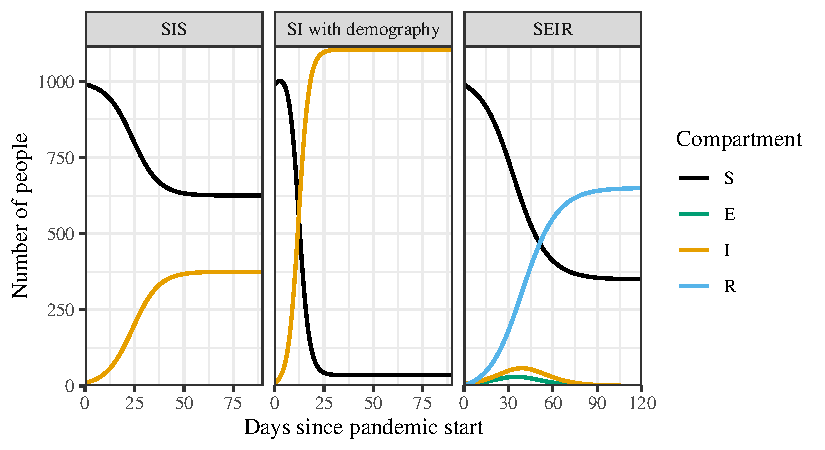
\includegraphics{ODE_plots.pdf}
    \caption[{
        $SIS,$ $SI$ with demography, and $SEIR$ deterministic 
        ODE model simulations
    }]{
        Solutions to the ODEs describing the models
        depicted in Figure \ref{fig:simple_models}. The initial infectious
        population was $I_0 = 10,$ with $S_0 = 990.$ In the $SEIR$ model,
        $E_0 = R_0 = 0.$ For all models, $\beta = 0.4.$ For the $SIS$ and $SI$
        model with demography, $\gamma = 1/4.$ For the $SI$ model with
        demography, $\mu = 0.012$ and $\nu = 0.0012.$ For the $SEIR$ model,
        $\gamma = 1/90$ and $\sigma = 1/2.$
    }
    \label{fig:ODE_outputs}
\end{figure}

After specifying the initial conditions $S_0,$ $I_0$, and so forth,
the ODEs can be numerically solved. Figure \ref{fig:ODE_outputs} shows
solutions to the three models introduced so far for an initial population
$N_0 = 1000$, with an initial infectious population $I_0 = 10.$ Under the
models without demography, $N_t$ remains constant. The disease is eradicated
for the $SEIR$ model after a small case spike. The disease reaches a
steady state equilibrium for the $SIS$ and
$SI$ with demography model, with a much higher number of infected individuals
in the $SI$ with demography model, since once an individual acquires the
disease, they have it until they die.

\section{Stochastic Models}

\subsection*{Motivating the Form of the Stochastic Model}

Deterministic ODE models can be appropriate to study infectious diseases
when the disease is near equilibrium and the numbers
in each compartment are large. At the start of an epidemic, when the
number of infected individuals is small, the behaviour of the epidemic may
vary significantly. When case numbers are small, there is a non-zero
probability that the disease may die out, but under the right conditions,
such as a large gathering of people
in a small space, the outbreak may become a pandemic.
In these cases, a deterministic model is inadequate in emulating real-world
behaviour. For this reason, we consider stochastic models of disease.
A natural stochastic analogue for a deterministic
model can be constructed considering
Poisson point processes and their properties.

\begin{definition}[Poisson Point Process]\label{def:ppp}
    $\{\N(t)\}_{t\geq0}$ is a \bemph{(stationary) Poisson point process} with 
    intensity $\kappa$ if \begin{enumerate}
        \item $\N(0) = 0$
        \item $\N(t_1) - \N(t_0), 
        \N(t_2) - \N(t_1), \dots, \N(t_n) - \N(t_{n-1})$ 
        are independent for $0 \leq t_0 < t_1 < \dots < t_{n-1} < t_n $
        \item $\N(t_2) - \N(t_1) 
        \sim \Pois(\kappa(t_2 - t_1)), 0 \leq t_1 < t_2.$
    \end{enumerate}
\end{definition}

To demonstrate how Poisson point processes aid us in creating a natural
analogue of the deterministic model, we construct two Poisson processes
that, when combined, have the
the same instantaneous average behaviour as the
deterministic ODE model.

Consider the deterministic $SIS$ model described by Equations
\ref{eq:SIS_1} and \ref{eq:SIS_2} at time $t^*.$ The
instantaneous rate at which $S_t$ is decreasing is
$\beta \frac{I_{t^*}}{N} S_{t^*}.$ In other words, at time $t^*,$
an individual leaves
the susceptible compartment every $\beta \frac{I_{t^*}}{N} S_{t^*}$
units of time.

Now consider a Poisson point process $\{\N_1(t - t^*)\}_{t\geq t^*}$ with
intensity $\beta \frac{I_{t^*}}{N} S_{t^*}$ corresponding to the count of the
number of individuals who have left $S$ and entered $I$ $t$ units of time
since $t^*.$ The average rate at which an individual leaves $S$ is then
\begin{align*}
    \frac{\diff \E(\N_1(t^*))}{\diff t^*}
    = & \lim_{\delta \to 0}\frac{\E{(\N(t^* + \delta) - \N(t^*))}}{\delta}
    \tag{Since the mean of a Poisson random variable is its intensity}     \\
    = & \frac{
        \beta \frac{I_{t^*}}{N} S_{t^*}
        (t^* + \delta - t^*)
        \beta \frac{I_{t^*}}{N} S_{t^*}
    }{
        \delta
    }                                                                      \\
    = & \beta \frac{I_{t^*}}{N} S_{t^*},
\end{align*}
the same rate as the ODE model.

Under the same deterministic ODE formulation of the $SIS$ model,
the instantaneous
rate into $S$ at time $t^*$ is $\gamma I_{t^*}.$ Also, as above, we
construct a Poisson point process $\{\N_2(t - t^*)\}_{t\geq t^*}$ with
mean rate $\gamma I_{t^*}$ describing the number of recoveries from
$I$ to $S$
since
$$\frac{\diff \E(\N_2(t^*))}{\diff t^*} = \gamma I_{t^*}.
$$

Combining the two processes, we can see that the rate of change in the
average number of people in $S$ is
$$
    \frac{\diff \E(\N_2(t^*) - \N_1(t^*))}{\diff t^*}
    = \frac{\diff \E(\N_2(t^*)) - \diff \E(\N_1(t^*))}{\diff t^*}
    = -\beta \frac{I_t}{N}S_t + \gamma I
    = \frac{\diff S_t}{\diff t}.
$$

We can model each
transition as a Poisson point process for an 
arbitrary number of compartments and transitions

Therefore, we construct a stochastic analogue for the ODEs in the following way.
Let the stochastic model be a
random vector
$\{\mathbf{C}_t\}_{t\geq 0} = \{C_1(t), C_2(t), \dots, C_n(t)\}_{t\geq 0}$
where $C_i:\mathbb{R} \to \mathbb{N}\cup\{0\},$ is the number of people in
compartment $C_i,$ and for any fixed $t$, $\{C_1(t), C_2(t), \dots, C_n(t)\}$
is a random variable describing the state of the model. For example, the $SI$
with demography model can be represented as
$\{\mathbf{C}_t\}_{t\geq 0}:=\{S_t, I_t\}_{t\geq 0}.$
% $\{\mathbf{C}_t\}_{t\geq 0}$ is a continuous time Markov chain 
% with transition kernel corresponding to 
% the rates of the model. 
% For example, in the $SI$ model with demography in 
% Figure \ref{fig:SI_demog_model} the transition rates are: \begin{itemize}
%     \item $\{s, i\}$ to $\{s + 1, i\}$ has rate $\mu (s + i)$
%     \item $\{s, i\}$ to $\{s - 1, i\}$ has rate $\nu s$
%     \item $\{s, i\}$ to $\{s - 1, i + 1\}$ has rate $\beta \frac{i}{i+s}s$
%     \item $\{s, i\}$ to $\{s, i - 1\}$ has rate $(\nu + \gamma) i.$
% \end{itemize}

If the model is in state $\{S_t, I_t\},$ after the next transition
at time $t^*,$ the next possible states are:
\begin{enumerate}
    \item $\{S_{t^*}, I_{t^*}\}=\{S_t + 1, I_t\}$ %with rate $\mu (S_t + I_t)$
    \item $\{S_{t^*}, I_{t^*}\}=\{S_t - 1, I_t\}$ %has rate $\nu S_t$
    \item $\{S_{t^*}, I_{t^*}\}=\{S_t - 1, I_t + 1\}$ %has rate $\beta \frac{I_t}{I_t+S_t}S_t$
    \item $\{S_{t^*}, I_{t^*}\}=\{S_t, I_t - 1\}.$ %has rate $(\nu + \gamma) I_t.$
\end{enumerate}

Each of these transitions behaves like Poisson processes at time $t.$ We think
of these processes in the following way:
\begin{itemize}
    \item $\{\mathcal{E}_1(t^*)\}_{t^*\geq 0}:$
          the number of births into $S$ after time $t$ with intensity
          $\mu N_{t}$
    \item $\{\mathcal{E}_2(t^*)\}_{t^*\geq 0}:$
          the number of deaths in $S$ after time $t$ with intensity
          $\nu S_{t}$
    \item $\{\mathcal{E}_3(t^*)\}_{t^*\geq 0}:$
          the number of infections after time $t$ with intensity
          $\beta \frac{I_{t}}{N_{t}} S_{t}$
    \item $\{\mathcal{E}_4(t^*)\}_{t^*\geq 0}:$
          the number of deaths from $I$ after time $t$ with intensity
          $(\nu + \gamma) I_{t}.$
\end{itemize}

Since the sum of two Poisson point processes is a Poisson point process (see
Theorem \ref{thm:sum_ppp}), the time between events in a Poisson process
is exponentially distributed (see Theorem \ref{thm:next_pp_event})
then
$$
    \{\mathcal{E}(t)\}_{t\geq 0}:=\{\mathcal{E}_1(t) + \mathcal{E}_2(t)
    + \mathcal{E}_3(t) + \mathcal{E}_4(t)\}_{t\geq 0}
$$
is a Poisson point process with intensity
$$\mu N_{t^*} + \nu S_{t^*} + \beta \frac{I_{t^*}}{N_{t^*}} S_{t^*}
    + (\nu + \gamma) I_{t^*}.$$
The time until the next transition is exponentially distributed
$$
    \Exp(\mu N_{t^*} + \nu S_{t^*}
    + \beta \frac{I_{t^*}}{N_{t^*}} S_{t^*} + (\nu + \gamma) I_{t^*}).
$$

Therefore, simulating the time to the next transition, given
the current number of individuals in each compartment, simply involves
simulating from an exponential distribution. 
Theorem \ref{thm:which_ppp} states that 
given that a transition occurred, the probability it was due to 
the process
$\mathcal{E}_i$ is proportional to its intensity. As soon as the transition
occurs, all the intensities for each Poisson process will be updated since
the intensities depend on the number of individuals in each compartment.

\subsection*{Doob-Gillespie Algorithm}

\begin{algorithm}[htbp]
    \caption[{
        The Doob-Gillespie Algorithm
    }]{
        The Doob-Gillespie Algorithm \parencite{gillespie_exact_1977}
        }\label{alg:doob}
    \begin{algorithmic}
        \State Initialise time $t \gets 0$ and initial state of the model $\mathbf{C}(0) := \{C_1(0), C_2(0), \dots, C_n(0)\}$
        \While{termination condition not met}
        \State Calculate intensities $\kappa_i$ for all possible events $\mathcal{E}_i$
        \State Calculate total intensity $\kappa = \sum_i \kappa_i$
        \State Generate $\Delta t \sim \Exp(\kappa)$
        \State Choose event $\mathrm{E}_i$ with probability $\frac{\kappa_i}{\kappa}$
        \State Update time $t \gets t + \Delta t$
        \State Update state of $\mathbf{C}(t + \delta t) \gets \mathbf{C}(t) + \text{ change in state due to event } \mathcal{E}_i$
        \EndWhile
    \end{algorithmic}
\end{algorithm}

This leads naturally to a standard method of simulating the stochastic 
model through Algorithm \ref{alg:doob}. 
The Doob-Gillespie algorithm 
exploits the local behaviour of the compartments as described, sampling
an exponential random variable, choosing an event with probabilities 
proportional to their intensities, updating the model, and updating the 
intensities given a 
set of starting conditions \parencite{gillespie_exact_1977}.

\begin{figure}[htbp]
    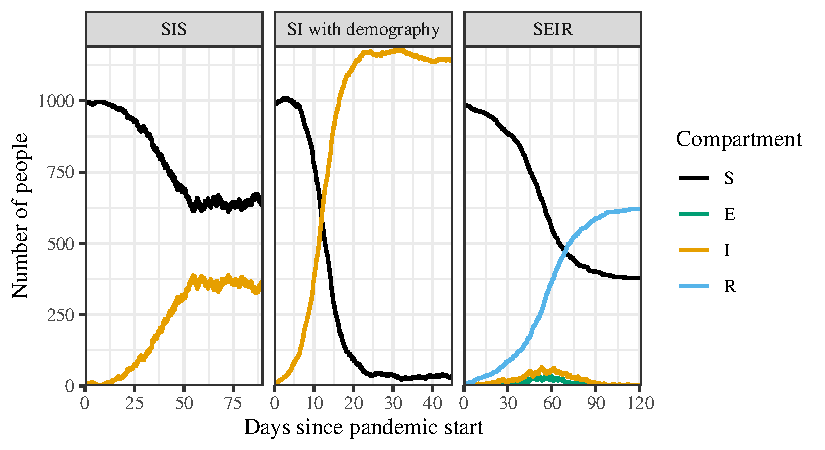
\includegraphics{doob_plots.pdf}
    \caption[{
        $SIS$, $SI$ with demography, and $SEIR$ Doob-Gillespie
        model simulations
    }]{
        Exact stochastic simulations of the three different models using 
        Algorithm \ref{alg:doob}. The parameters used were identical to 
        those in Figure \ref{fig:ODE_outputs}}
        \label{fig:doob_outputs}
\end{figure}

Figure \ref{fig:doob_outputs} demonstrates Doob-Gillespie simulations for the
models discussed in this chapter. Compared to the deterministic ODE simulations
in Figure \ref{fig:ODE_outputs}, the stochastic simulations still show variation
even near the equilibria.

\subsection*{\texorpdfstring{$\tau$}{Lg}-Leaping}

Because the Doob-Gillespie algorithm is an exact simulation method, 
when the 
intensities become large, or many people are infected, the time step
$\tau$ can become increasingly small, resulting in long simulations times.

$\tau$-leaping - Algorithm \ref{alg:tau_leaping} - further exploits the 
local Poisson point process-like behaviour of
epidemiological models \parencite{gillespie_approximate_2001}. 
Consider the $SIS$ model
when $S_t = I_t = 10000.$ Events happen at a very high rate, meaning 
the $\Delta t$ found in each step of the Doob-Gillespie algorithm will be 
very small, but the rates also change a negligible amount after each event 
(compare $\gamma\times 10000$ to $\gamma\times 10001$ or $\gamma\times 9999$). 
Therefore, we can approximate the number of events in a short time period 
$\tau$ as a Poisson point process with the total intensity 
$\kappa = \sum_i \kappa_i$ at time $t,$ with the probability of any one 
event having the same probability as above of $\frac{\kappa_i}{\kappa}.$ 
Therefore, we have the following algorithm.

\begin{algorithm}
    \caption[{
        $\tau$-Leaping Algorithm
        }]{
            $\tau$-Leaping Algorithm \cite{gillespie_approximate_2001}
            }
    \label{alg:tau_leaping}
    \begin{algorithmic}
        \State Initialise time $t \gets 0$ and initial state of the model $\mathbf{C}(0) := \{C_1(0), C_2(0), \dots, C_n(0)\}$
        \While{termination condition not met}
        \State Calculate intensities $\kappa_i$ for all possible events $\mathcal{E}_i$
        \State Calculate total intensity $\kappa = \sum_i \kappa_i$
        \State Choose a suitable time step $\tau$ (this can be deterministic or adaptive)
        \State Calculate Poisson random variable $X \sim \text{Poisson}(\kappa\tau)$
        \For{$i$ in 1 to $X$}
        \State Choose event $\mathrm{E}_i$ with probability $\frac{\kappa_i}{\kappa}$
        \State Update state of $\mathbf{C}(t + \tau) \gets \mathbf{C}(t) + \text{ change in state due to event } \mathcal{E}_i$
        \EndFor
        \State Update time $t \gets t + \tau$
        \EndWhile
    \end{algorithmic}
\end{algorithm}

% \section{Individual based models}